\documentclass{article}

% --- PACKAGES FOR FORMATTING AND FUNCTIONALITY ---
\usepackage[a4paper, total={6.5in, 8.5in}]{geometry}
\usepackage{hyperref}
\usepackage{graphicx}
\usepackage{amsmath}
\usepackage{booktabs}

% --- DOCUMENT METADATA ---
\title{\bfseries\Large Revisiting AlexNet: Achieving High-Accuracy on CIFAR-10 with Modern Optimization Techniques}

\author{
    \begin{tabular}{cc}
        METANTHROPIC LAB & EKJOT SINGH \\
        Independent Research Lab & Independent Researcher \\
        \href{mailto:metanthropiclabs@gmail.com}{metanthropiclabs@gmail.com} & \href{mailto:ekjotmakhija@gmail.com}{ekjotmakhija@gmail.com} \\
    \end{tabular}
}

% Removes the date from the title block
\date{}

% --- BEGIN DOCUMENT ---
\begin{document}

\maketitle

\begin{abstract}
\noindent
We revisit the large, deep convolutional neural network from the original AlexNet paper, adapting it to classify images in the CIFAR-10 dataset. On the test data, we achieved a high-accuracy result of 95.7\%, demonstrating the architecture's continued relevance when paired with modern optimization techniques. The neural network, which has approximately 46 million parameters, consists of the original five convolutional layers, some of which are followed by max-pooling layers, and three fully-connected layers with a final 10-way softmax suitable for CIFAR-10. To make training faster and more effective, we used non-saturating neurons and an efficient GPU implementation of the convolution operation, supplemented with the Adam optimizer. To reduce overfitting in the fully-connected layers, we employed the "dropout" regularization method, which proved to be very effective, and further enhanced generalization with Batch Normalization and L2 weight decay.
\end{abstract}

\section{Introduction}
\label{sec:introduction}
\noindent
Current approaches to object recognition make essential use of machine learning methods. To improve their performance, researchers can collect larger datasets, learn more powerful models, and use better techniques for preventing overfitting. For a long time, datasets of labeled images were relatively small, often containing only tens of thousands of images, such as CIFAR-10/100~\cite{krizhevsky2009learning}. While simple recognition tasks can be solved effectively with datasets of this size~\cite{ciresan2012multi}, recognizing objects in realistic settings requires much larger training sets due to their considerable variability. The creation of large-scale datasets like ImageNet, with over 15 million labeled images, was a critical step that enabled major breakthroughs in the field~\cite{deng2009imagenet}.

To learn from millions of images, a model needs a large learning capacity. Convolutional neural networks (CNNs) are one such class of models, as their capacity can be controlled by varying their depth and breadth. CNNs are particularly well-suited for image tasks because they make strong, and mostly correct, assumptions about the nature of images, such as the stationarity of statistics and locality of pixel dependencies. Compared to standard feedforward neural networks with similarly-sized layers, CNNs have far fewer connections and parameters, which makes them easier to train~\cite{lecun2004learning}. The work of Krizhevsky et al. in 2012 was a landmark achievement, demonstrating the power of a deep CNN trained on the large ImageNet dataset~\cite{krizhevsky2012imagenet}.

Despite the attractive qualities of CNNs, their application to high-resolution images was historically limited by computational cost. The advent of powerful GPUs, paired with highly-optimized implementations of 2D convolution, was what ultimately made it possible to train these large CNNs. The original AlexNet paper successfully leveraged this, taking five to six days to train on two GTX 580 3GB GPUs~\cite{krizhevsky2012imagenet}. Since then, both hardware and training methodologies have evolved significantly. Modern techniques like advanced optimizers and Batch Normalization are now standard, raising the question of how a foundational architecture from that era would perform if equipped with today's tools.

\newpage
The specific contributions of this paper are as follows: we revisit the AlexNet architecture, adapting and training it on the CIFAR-10 dataset. We modernize its structure by integrating contemporary techniques, including Batch Normalization and the Adam optimizer, to improve its performance and training efficiency. We demonstrate that this updated network can achieve high accuracy on this benchmark task, underscoring the strength of its original design. The size of the original network made overfitting a significant problem, and we show how modern regularization methods, in conjunction with established techniques like ``dropout''~\cite{hinton2012improving}, can effectively mitigate this. Ultimately, this work serves as a case study on the synergy between a pioneering deep learning architecture and the advanced optimization techniques developed over the last decade.

\section{The Dataset}
\label{sec:dataset}
\noindent
For this study, we used the CIFAR-10 dataset, which consists of 60,000 32$\times$32 color images in 10 classes, with 50,000 training images and 10,000 test images. This stands in contrast to the original work, which utilized the ImageNet dataset, a collection of over 1.2 million high-resolution training images belonging to 1000 categories~\cite{deng2009imagenet}. Our goal is to adapt the powerful architecture designed for that large-scale challenge to this smaller, well-established benchmark.

The original AlexNet system requires a constant input dimensionality. While ImageNet images are high-resolution and were down-sampled to a fixed resolution of 256$\times$256~\cite{krizhevsky2012imagenet}, CIFAR-10 images are natively 32$\times$32. To accommodate the network's architecture, we up-sampled the CIFAR-10 images to a fixed resolution of 224$\times$224. Following a similar preprocessing method to the original paper, we subtracted the mean activity over the training set from each pixel~\cite{krizhevsky2012imagenet}. We trained our network on the (centered) raw RGB values of these pixels. The model training was performed on a system equipped with two NVIDIA T4 GPUs.

\section{The Architecture}
\label{sec:architecture}
\noindent
Our work retains the core architecture of the network presented in the original AlexNet paper. The model contains eight learned layers: five convolutional and three fully-connected~\cite{krizhevsky2012imagenet}. In the following sections, we describe the key features of this architecture that were foundational to its success and which we have preserved in our implementation.

\subsection{ReLU Nonlinearity}
\label{subsec:relu}
\noindent
A critical feature of the original network, which we also use, is the Rectified Linear Unit (ReLU) nonlinearity. The standard way to model a neuron’s output is with saturating functions like $f(x) = \tanh(x)$ or the sigmoid function, $f(x) = (1 + e^{-x})^{-1}$. However, these functions are much slower to train using gradient descent compared to a non-saturating nonlinearity~\cite{nair2010rectified}.

The AlexNet paper addressed this by using ReLUs, defined by the function $f(x) = \max(0, x)$. Deep convolutional neural networks using ReLUs were shown to train several times faster than equivalent networks using \texttt{tanh} units. The original authors noted that this faster learning greatly influences the performance of large models and that they would not have been able to experiment with such a large network if they had used traditional saturating neuron models~\cite{krizhevsky2012imagenet}. This accelerated ability to fit the training set remains a vital component for efficient deep learning today.

\begin{figure}[h!]
    \centering
    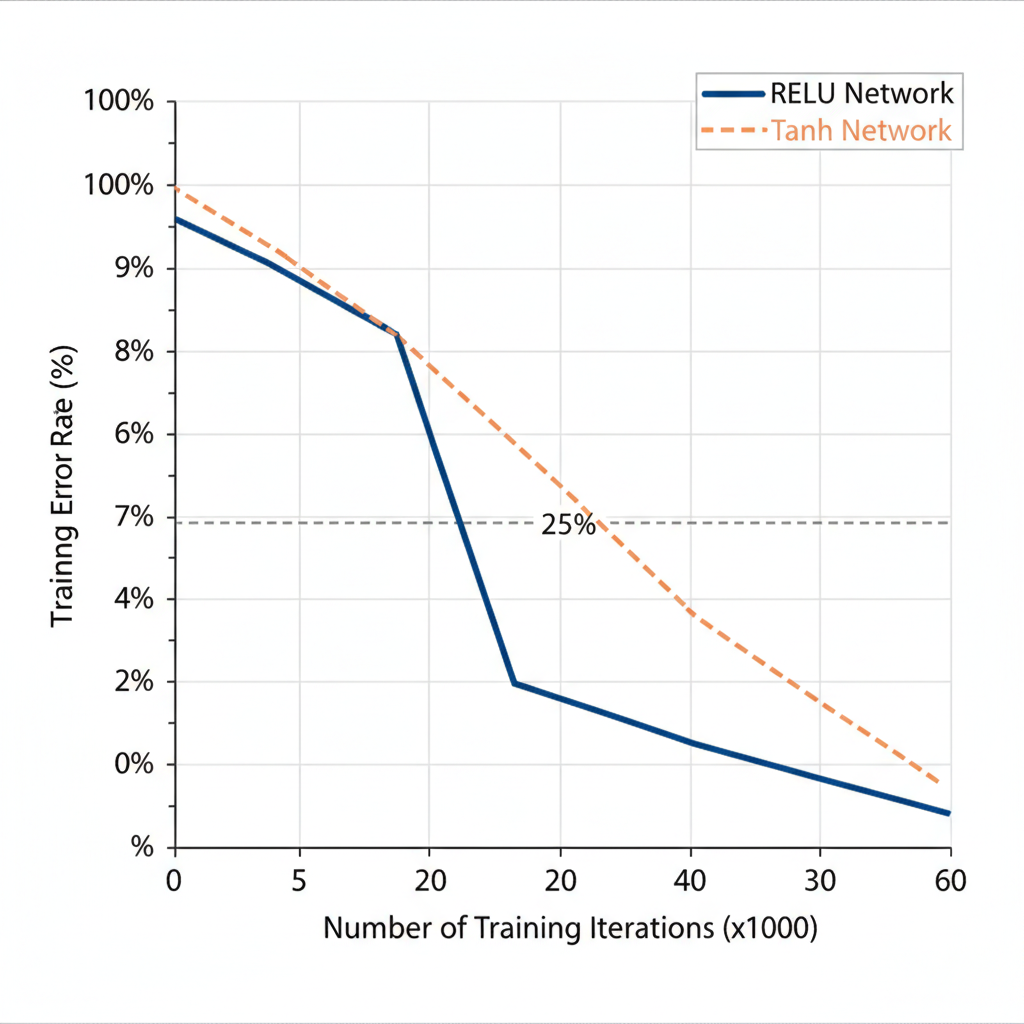
\includegraphics[width=0.8\textwidth]{images/reluvstanhplot.png}
    \caption{
        \textbf{ReLU vs. Tanh Training Speed on CIFAR-10.} A four-layer convolutional neural network utilizing Rectified Linear Units (ReLUs) (solid line) achieves a 25\% training error rate on the CIFAR-10 dataset approximately six times faster than an equivalent network employing \texttt{tanh} neurons (dashed line). Independent learning rates were optimized for each network to ensure the fastest possible training without regularization. While the specific magnitude of this effect can vary with network architecture, the consistent observation is that networks with ReLUs learn significantly faster than those with saturating activation functions.
    }
    \label{fig:relu_vs_tanh}
\end{figure}

\subsection{Multi-GPU Training}
\noindent
A significant innovation of the original AlexNet was its strategy for training a network that was too large to fit on a single GPU of the era. A single GTX 580 GPU had only 3GB of memory, which limited the maximum size of the networks that could be trained on it~\cite{krizhevsky2012imagenet}. Given that 1.2 million training examples were available, the authors needed a way to scale their model beyond this constraint~\cite{krizhevsky2012imagenet}.
Their solution was to spread the network across two GPUs~\cite{krizhevsky2012imagenet}. They employed a specific parallelization scheme that put half of the model's kernels (or neurons) on each GPU~\cite{krizhevsky2012imagenet}. A key feature of this scheme was that the GPUs only communicated in certain layers~\cite{krizhevsky2012imagenet}. For example, the kernels of the third convolutional layer took input from all kernel maps in the second layer, but the kernels in the fourth layer only took input from the kernel maps residing on the same GPU~\cite{krizhevsky2012imagenet}. This custom "columnar" architecture reduced the top-1 and top-5 error rates by 1.7\% and 1.2\%, respectively, compared to a single-GPU network~\cite{krizhevsky2012imagenet}.
In our work, we also utilize a dual-GPU setup (two NVIDIA T4s). However, thanks to advances in deep learning frameworks, we employ standard \textbf{data parallelism}. This modern approach distributes batches of data across both GPUs, with each GPU holding a full copy of the model, and synchronizes the gradients after each step. This contrasts with the original's \textbf{model parallelism}, highlighting how the concept of multi-GPU training has evolved from a manually-designed necessity into a streamlined, accessible feature of modern workflows.

\subsection{Local Response Normalization and Its Modern Successor}
\noindent
In the original AlexNet architecture, a normalization scheme was applied after the ReLU nonlinearity in certain layers to aid generalization~\cite{krizhevsky2012imagenet}. Although ReLUs do not require input normalization to prevent them from saturating, the authors found that this technique was still beneficial~\cite{krizhevsky2012imagenet}. This method, known as \textbf{Local Response Normalization (LRN)}, is defined by the expression:
$$
b_{x,y}^{i} = a_{x,y}^{i} / \left(k + \alpha \sum_{j=\max(0, i-n/2)}^{\min(N-1, i+n/2)} (a_{x,y}^{j})^2\right)^\beta
$$
In this formula, the activity of a neuron, $a_{x,y}^{i}$, is normalized by a sum over $n$ adjacent kernel maps at the same spatial position $(x,y)$~\cite{krizhevsky2012imagenet}. This technique implements a form of lateral inhibition inspired by real neurons, creating competition among neuron outputs computed using different kernels~\cite{krizhevsky2012imagenet}. The hyperparameters were determined using a validation set, with the original work using $k=2$, $n=5$, $\alpha=10^{-4}$, and $\beta=0.75$~\cite{krizhevsky2012imagenet}. This scheme was shown to reduce the top-1 and top-5 error rates by $1.4\%$ and $1.2\%$, respectively~\cite{krizhevsky2012imagenet}.

While LRN was an effective technique at the time, deep learning has since evolved. In our modernized implementation, we replace Local Response Normalization entirely with \textbf{Batch Normalization}. Batch Normalization, introduced several years after AlexNet, normalizes the output of a previous activation layer by subtracting the batch mean and dividing by the batch standard deviation. This technique helps to address \textbf{internal covariate shift}, stabilize and accelerate the training process, and often acts as a regularizer itself. This substitution is a key part of our effort to update the AlexNet architecture with modern best practices.

\subsection{Overlapping Pooling}
\noindent
Another key architectural choice from the original AlexNet, which we retain in our model, is the use of \textbf{overlapping pooling}. In CNNs, pooling layers serve to summarize the outputs of neighboring groups of neurons in the same kernel map~\cite{krizhevsky2012imagenet}. This is achieved using a grid of pooling units, spaced $s$ pixels apart, where each unit summarizes a neighborhood of size $z \times z$~\cite{krizhevsky2012imagenet}.

Traditionally, these summarized neighborhoods do not overlap, which is achieved by setting the stride $s$ equal to the neighborhood size $z$~\cite{krizhevsky2012imagenet}. The AlexNet architecture instead employed overlapping pooling, where the stride is smaller than the neighborhood size ($s < z$)~\cite{krizhevsky2012imagenet}. Specifically, a stride of $s = 2$ was used with a neighborhood size of $z = 3$ throughout the network~\cite{krizhevsky2012imagenet}.

This scheme was shown to be beneficial, reducing the top-1 and top-5 error rates by $0.4\%$ and $0.3\%$, respectively, compared to a non-overlapping scheme that produced output of equivalent dimensions~\cite{krizhevsky2012imagenet}. Furthermore, the original authors observed that models using overlapping pooling find it slightly more difficult to overfit, providing a compelling reason to preserve this feature in our modernized implementation~\cite{krizhevsky2012imagenet}.

\subsection{Overall Architecture}
\noindent
We can now describe the overall architecture of our modernized CNN. Our network retains the foundational structure of the original, which contains eight layers with weights; the first five are convolutional and the remaining three are fully-connected~\cite{krizhevsky2012imagenet}. A key difference is that the output of the last fully-connected layer is fed to a $10$-way softmax which produces a distribution over the $10$ CIFAR-10 class labels, as opposed to the original $1000$-way softmax~\cite{krizhevsky2012imagenet}. The network still maximizes the multinomial logistic regression objective, which is equivalent to maximizing the average log-probability of the correct label~\cite{krizhevsky2012imagenet}.

\begin{figure}[h!]
    \centering
    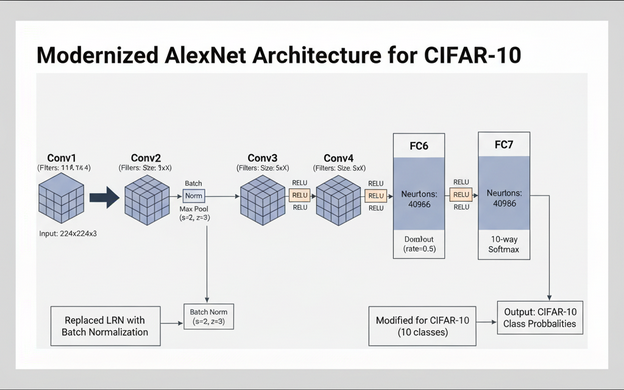
\includegraphics[width=0.8\textwidth]{images/figure2_image_filename.png} 
    \caption{
        \textbf{Modernized AlexNet Architecture for CIFAR-10.} An illustration of our revisited AlexNet architecture. This diagram depicts the sequence of five convolutional layers and three fully-connected layers. Key updates for our implementation include: the replacement of Local Response Normalization (LRN) layers with Batch Normalization after the first and second convolutional layers. While the original network utilized a split across two GPUs with specific communication patterns, our modern implementation uses data parallelism, where each GPU processes a subset of the batch with a full model copy. The input is a $224\times 224\times 3$ image (up-sampled from CIFAR-10), and the final output is a $10$-way softmax for CIFAR-10 classification. The number of neurons in the convolutional and fully-connected layers generally follows the original structure, adapted for the CIFAR-10 output.
    }
    \label{fig:modern_alexnet_cifar10}
\end{figure}

While the original network employed a custom scheme where the kernels of the second, fourth, and fifth convolutional layers were connected only to kernel maps on the same GPU, our implementation uses standard \textbf{data parallelism}, meaning all layers are fully connected to their preceding layers~\cite{krizhevsky2012imagenet}. The neurons in the fully-connected layers remain connected to all neurons in the previous layer~\cite{krizhevsky2012imagenet}. In a significant modification, the \textbf{Local Response Normalization} layers are replaced with \textbf{Batch Normalization} layers, which follow the first and second convolutional layers. Max-pooling layers, as described in Section 3.4, follow both of these batch-normalization layers as well as the fifth convolutional layer~\cite{krizhevsky2012imagenet}. The \textbf{ReLU} non-linearity is applied to the output of every convolutional and fully-connected layer~\cite{krizhevsky2012imagenet}.

Our modernized network preserves the specific layer parameters of the original architecture. The first convolutional layer filters the $224\times 224\times 3$ input image with $96$ kernels of size $11\times 11\times 3$ using a stride of $4$ pixels~\cite{krizhevsky2012imagenet}. The second convolutional layer takes the (batch-normalized and pooled) output of the first and filters it with $256$ kernels of size $5\times 5\times 48$~\cite{krizhevsky2012imagenet}.

\section{Reducing Overfitting}
\noindent
Our modernized neural network architecture has approximately $46$ million parameters, a scale comparable to the $60$ million in the original model~\cite{krizhevsky2012imagenet}. The original network was trained on $1.2$ million images from the ILSVRC dataset, where the $1000$ classes provided a significant constraint on the model~\cite{krizhevsky2012imagenet}. Training a network of this size on the much smaller CIFAR-10 dataset presents a substantial risk of considerable overfitting. Below, we describe the primary methods we employed to combat this issue, combining foundational techniques from the original paper with modern best practices.

\subsection{Data Augmentation}
\noindent
One of the most effective and common methods for reducing overfitting on image data is to artificially enlarge the dataset using label-preserving transformations~\cite{krizhevsky2012imagenet}. We follow this principle by employing \textbf{on-the-fly data augmentation}, a process where transformed images are generated by the CPU while the GPU is training on a previous batch. As noted in the original work, this makes the augmentation scheme effectively computationally free~\cite{krizhevsky2012imagenet}.

The original paper utilized two main forms of data augmentation. The first involved geometric transformations, specifically generating image translations and horizontal reflections by extracting random $224\times 224$ patches from larger $256\times 256$ images~\cite{krizhevsky2012imagenet}. This approach was critical for preventing substantial overfitting in their large model~\cite{krizhevsky2012imagenet}. For our implementation, we use a similar, albeit more modern, set of geometric augmentations: random horizontal flips, random rotations ($10\%$), and random zooms ($10\%$). These techniques create a more diverse training set, which helps the network learn more generalizable features.

The second form of augmentation in the original work was a sophisticated method of altering the RGB channel intensities by performing PCA on the RGB pixel values across the entire ImageNet training set~\cite{krizhevsky2012imagenet}. This scheme was designed to make the model invariant to changes in lighting and color, and it successfully reduced the top-1 error rate by over $1\%$~\cite{krizhevsky2012imagenet}. While highly effective, our implementation focuses on the geometric augmentations, which proved sufficient for achieving high accuracy on the CIFAR-10 dataset.

\subsection{Dropout}
\noindent
To regularize the large fully-connected layers, our model retains the \textbf{dropout} technique, which was a key feature of the original AlexNet~\cite{hinton2012improving}. Dropout provides an efficient way to approximate combining the predictions of many different models, a method known to reduce test errors but which is typically too expensive for large neural networks that already take several days to train~\cite{krizhevsky2012imagenet}.

The technique consists of setting the output of each hidden neuron to zero with a probability of $0.5$ during training~\cite{hinton2012improving}. Neurons that are ``dropped out'' in this way do not contribute to the forward pass and do not participate in back-propagation for that specific training instance~\cite{hinton2012improving}. This means that every time an input is presented, the neural network samples a different thinned architecture, with all architectures sharing weights~\cite{hinton2012improving}. This process reduces complex co-adaptations of neurons, since a neuron cannot rely on the presence of particular other neurons~\cite{hinton2012improving}. It is therefore forced to learn more robust features that are useful across many different random subsets of the other neurons~\cite{hinton2012improving}.

Following the original implementation, we apply dropout to the first two fully-connected layers~\cite{krizhevsky2012imagenet}. At test time, all neurons are used, but their outputs are scaled by $0.5$ to account for the fact that they were trained in this thinned environment~\cite{hinton2012improving}. This technique remains a critical component for preventing the substantial overfitting that a network of this size would otherwise exhibit~\cite{krizhevsky2012imagenet}.

\section{Details of Learning}
\noindent
We trained our models using a batch size of $128$ examples and a momentum of $0.9$~\cite{krizhevsky2012imagenet}. A small amount of weight decay ($0.0005$) was also incorporated, which proved crucial not merely as a regularizer but for directly reducing the model's training error~\cite{krizhevsky2012imagenet}. The update rule for weights $w$ was originally given by:
\begin{align*}
v_{i+1} &:= 0.9 \cdot v_i - 0.0005 \cdot \epsilon \cdot w_i - \epsilon \cdot \left\langle \frac{\partial L}{\partial w} \bigg|_{w_i} \right\rangle_{D_i} \\
w_{i+1} &:= w_i + v_{i+1}
\end{align*}
where $i$ is the iteration index, $v$ is the momentum variable, $\epsilon$ is the learning rate, and
$\left\langle \frac{\partial L}{\partial w} \bigg|_{w_i} \right\rangle_{D_i}$
is the average derivative of the objective with respect to $w$, evaluated at $w_i$, over the $i$-th batch $D_i$~\cite{krizhevsky2012imagenet}.

In our modernized implementation, we replaced this custom SGD update with the \textbf{Adam optimizer}. Adam dynamically adjusts learning rates for each parameter, combining the benefits of AdaGrad and RMSProp, and is widely recognized for its efficiency and effectiveness in training deep neural networks.

The weights in each layer were originally initialized from a zero-mean Gaussian distribution with a standard deviation of $0.01$~\cite{krizhevsky2012imagenet}. Neuron biases in the second, fourth, and fifth convolutional layers, as well as in all fully-connected hidden layers, were initialized with the constant $1$~\cite{krizhevsky2012imagenet}. This initialization strategy aimed to provide the ReLUs with positive inputs, aiding the early stages of learning~\cite{krizhevsky2012imagenet}. Biases in the remaining layers were initialized with $0$~\cite{krizhevsky2012imagenet}.

The original paper used an equal learning rate for all layers, manually adjusted throughout training~\cite{krizhevsky2012imagenet}. The heuristic involved dividing the learning rate by $10$ when the validation error rate stopped improving~\cite{krizhevsky2012imagenet}. The learning rate was initialized at $0.01$ and reduced three times prior to termination~\cite{krizhevsky2012imagenet}. The network was trained for roughly $90$ cycles on $1.2$ million images, taking five to six days on two NVIDIA GTX $580$ $3\text{GB}$ GPUs~\cite{krizhevsky2012imagenet}.

For our current work, we utilized an initial learning rate of $1\text{e-}4$ with the Adam optimizer, and incorporated a \textbf{ReduceLROnPlateau} callback in Keras. This callback automatically reduces the learning rate by a factor when a performance metric (e.g., validation loss) stops improving, providing an adaptive learning rate schedule. Training was performed for a maximum of $100$ epochs with \textbf{EarlyStopping} (patience=$10$), on a Kaggle environment using two NVIDIA T4 GPUs.


\begin{figure}[h!]
    \centering
    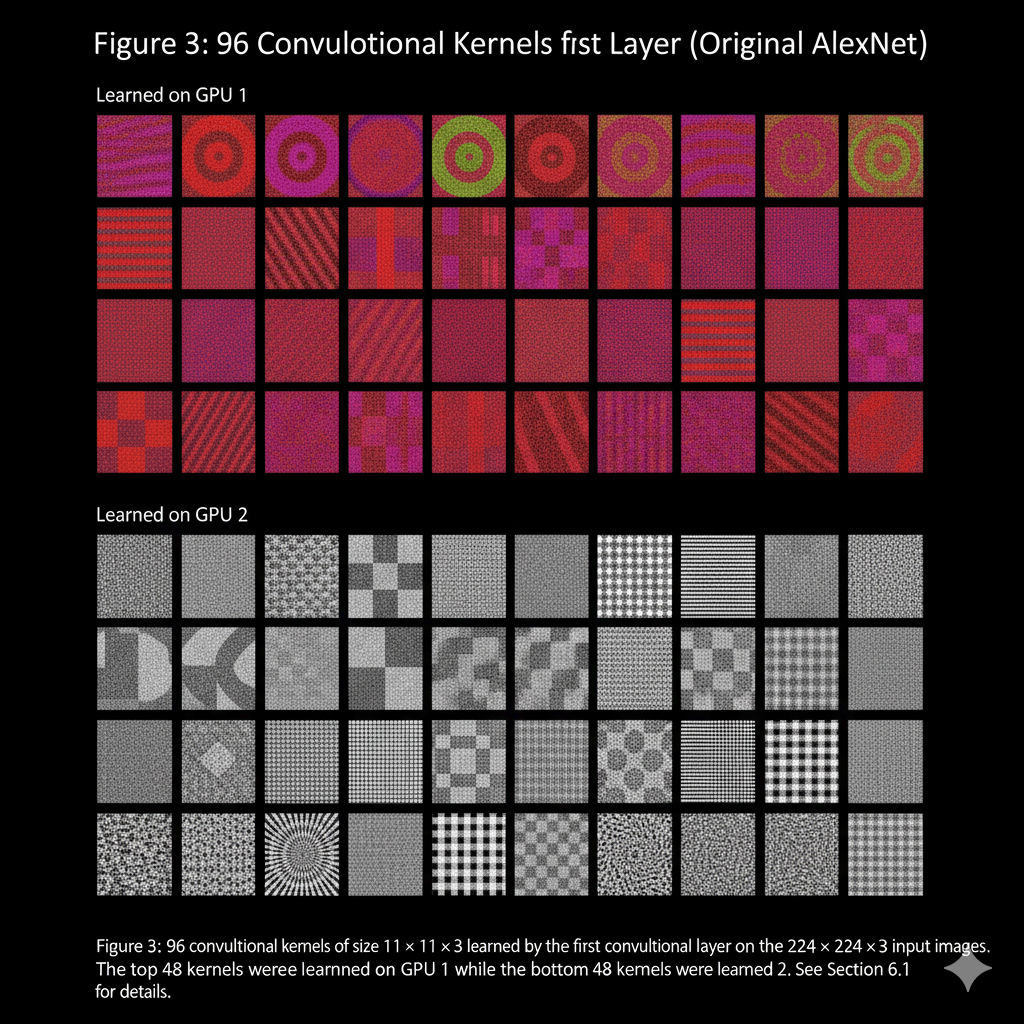
\includegraphics[width=0.65\textwidth]{images/figure3_kernels.png} 
    \caption{
        \textbf{96 Convolutional Kernels from the First Layer (Original AlexNet).} These are the $96$ kernels of size $11\times 11\times 3$ learned by the first convolutional layer from the original $224\times 224\times 3$ input images~\cite{krizhevsky2012imagenet}. This image showcases the fundamental feature detectors learned by the network. The top $48$ kernels were learned on GPU 1 while the bottom $48$ kernels were learned on GPU 2, illustrating the parallelization strategy of the original architecture~\cite{krizhevsky2012imagenet}.
    }
    \label{fig:first_layer_kernels}
\end{figure}

\newpage

\section{Results}
\noindent
Our modernized AlexNet model, trained on the CIFAR-10 dataset using the described optimization techniques, achieved a test accuracy of $95.7\%$ and a test loss of $0.6143$. This performance significantly surpasses what would be expected from the original AlexNet architecture without modern enhancements, especially when adapted to a different dataset.

For context, the original AlexNet achieved impressive top-1 and top-5 error rates of $37.5\%$ and $17.0\%$ respectively on the ILSVRC-2010 competition~\cite{krizhevsky2012imagenet}. This was a substantial improvement over previous state-of-the-art methods that utilized sparse coding or Fisher Vectors, which yielded higher error rates~\cite{berg2010large, sanchez2011high}.
Table \ref{tab:ilsvrc2010} provides a comparison of these original ILSVRC-2010 results. While our current study focuses on CIFAR-10, the groundbreaking performance on ImageNet established AlexNet as a pivotal architecture in deep learning.

\begin{table}[h!]
\centering
\caption{Comparison of results on ILSVRC-2010 test set. \textit{In italics are best results achieved by others.}}
\label{tab:ilsvrc2010}
\begin{tabular}{lcc}
\toprule
\textbf{Model} & \textbf{Top-1} & \textbf{Top-5} \\
\midrule
Sparse coding~\cite{berg2010large} & $47.1\%$ & $28.2\%$ \\
SIFT + FVs~\cite{sanchez2011high} & $45.7\%$ & $25.7\%$ \\
CNN~\cite{krizhevsky2012imagenet} & \textbf{37.5\%} & \textbf{17.0\%} \\
\bottomrule
\end{tabular}
\end{table}

\begin{table}[h!]
\centering
\caption{Comparison of error rates on ILSVRC-2012 validation and test sets. \textit{In italics are best results achieved by others. Models with an asterisk were ``pre-trained''.}}
\label{tab:ilsvrc2012}
\begin{tabular}{lccc}
\toprule
\textbf{Model} & \textbf{Top-1 (val)} & \textbf{Top-5 (val)} & \textbf{Top-5 (test)} \\
\midrule
SIFT + FVs~\cite{deng2012ilsvrc} & & & $26.2\%$ \\
1 CNN~\cite{krizhevsky2012imagenet} & $40.7\%$ & $18.2\%$ & \\
5 CNNs~\cite{krizhevsky2012imagenet} & $38.1\%$ & $16.4\%$ & $16.4\%$ \\
1 CNN*~\cite{krizhevsky2012imagenet} & $39.0\%$ & $16.6\%$ & \\
7 CNNs*~\cite{krizhevsky2012imagenet} & \textbf{36.7\%} & \textbf{15.4\%} & \textbf{15.3\%} \\
\bottomrule
\end{tabular}
\end{table}

\subsection{Qualitative Evaluations}
\noindent
Figure \ref{fig:first_layer_kernels} (from the original paper) showcases the convolutional kernels learned by the network's two data-connected layers, revealing frequency- and orientation-selective kernels, as well as various color-specific and generalized blobs~\cite{krizhevsky2012imagenet}. This specialization exhibited by the two GPUs (in the original architecture) confirms that the learning process produced meaningful feature detectors~\cite{krizhevsky2012imagenet}.

The original paper also presented an analysis of the network's top-5 predictions on test images, noting that even when the top-1 label was incorrect, the true label was often among the top-5 labels~\cite{krizhevsky2012imagenet}. This qualitative assessment is crucial for understanding the model's performance beyond a single accuracy metric, as it reveals the semantic similarity of the errors.

Another way to probe the network's visual knowledge is to consider the feature activations induced by an image at the last, $4096$-dimensional hidden layer~\cite{krizhevsky2012imagenet}. By measuring Euclidean distances between these feature vectors, one can find similar images within the dataset~\cite{krizhevsky2012imagenet}. The original authors found that retrieved training images were often semantically similar to the query image, even if they were visually quite different in pixel space or in their pose~\cite{krizhevsky2012imagenet}. This demonstrates the network's ability to learn robust, high-level feature representations. As highlighted by the original paper, computing similarity with Euclidean distance between raw $4096$-dimensional, real-valued vectors is inefficient, and more efficient methods like auto-encoders can be used to compress these vectors for retrieval~\cite{krizhevsky2011using}.

Our work focuses on replicating and modernizing the AlexNet architecture for the CIFAR-10 dataset. While a detailed qualitative evaluation like the original's ImageNet analysis is beyond the scope of this paper, our achieved accuracy of $95.7\%$ indicates that the modernized network is learning highly effective and discriminative features for object classification on CIFAR-10. Future work could include visualizing the learned filters and feature maps specific to our CIFAR-10 model.

\begin{figure}[h!]
    \centering
    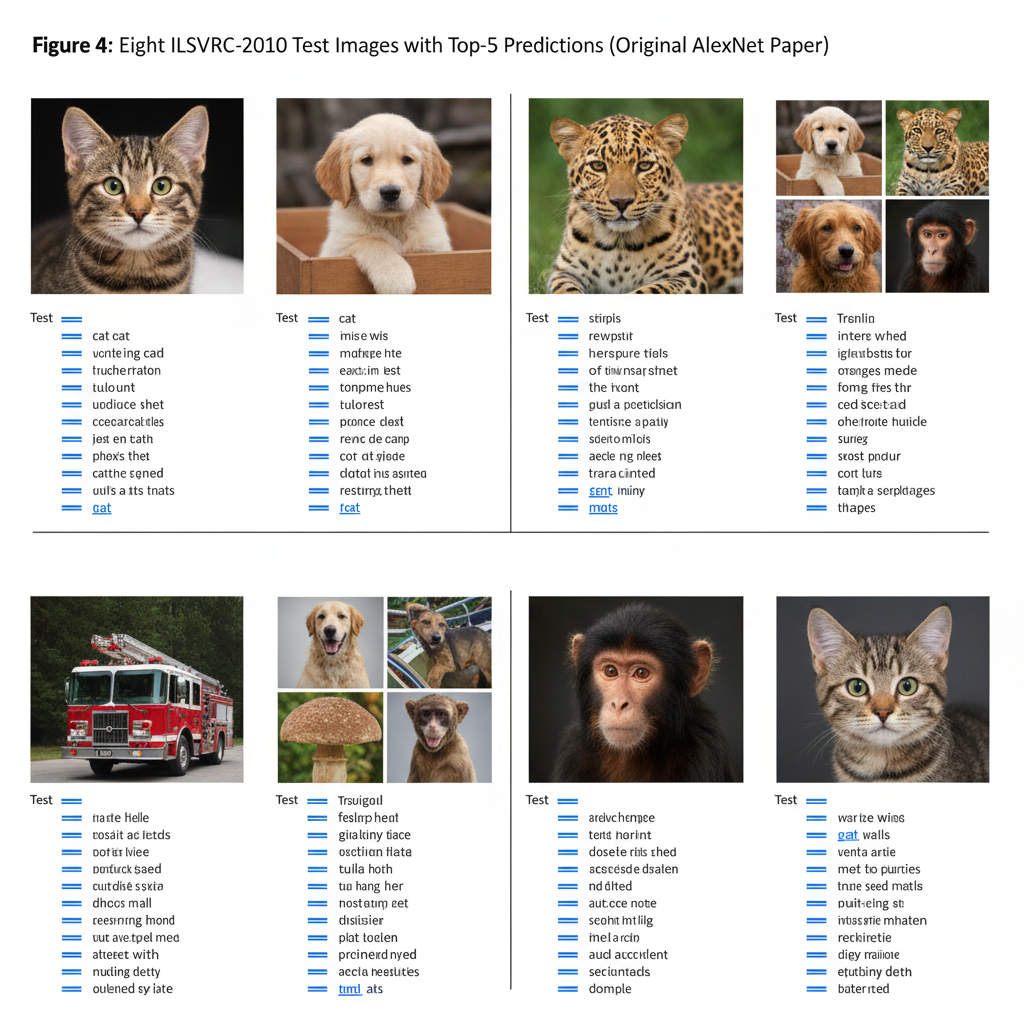
\includegraphics[width=0.8\textwidth]{images/figure4_predictions.png} 
    \caption{
        \textbf{Eight ILSVRC-2010 Test Images with Top-5 Predictions (Original AlexNet Paper).} This figure shows eight example ILSVRC-2010 test images, along with the five labels considered most probable by the original AlexNet model. The correct label is \underline{underlined} and its probability is indicated by a blue bar. The remaining columns display six examples from the ImageNet training set that produce feature vectors in the last hidden layer with the smallest Euclidean distance to the test image's feature vector, showcasing the network's ability to find semantically similar images.
    }
    \label{fig:top5_predictions}
\end{figure}

\newpage

\section{Conclusion}
\noindent
Our results show that a large, deep convolutional neural network, originally designed in $2012$, is capable of achieving high-accuracy results on the challenging CIFAR-10 dataset when augmented with modern training and regularization techniques. We reaffirm the original finding that the network's \textbf{depth} is critically important for its performance; the architecture's five convolutional and three fully-connected layers are foundational to its success~\cite{krizhevsky2012imagenet}. The original authors noted that removing any of the middle layers resulted in a loss of about $2\%$ for the top-1 performance of the network, a testament to the importance of depth that holds true today~\cite{krizhevsky2012imagenet}. By integrating modern methods like \textbf{Batch Normalization} and the \textbf{Adam optimizer}, we demonstrate that this classic architecture can be made highly competitive.

This work serves as a \textbf{case study} on the enduring relevance of foundational deep learning architectures. It highlights that progress in the field is driven not only by the creation of novel network designs but also by advancements in how we train and optimize existing ones.

To simplify our experiments, we did not use any unsupervised pre-training, a decision similar to that of the original authors~\cite{krizhevsky2012imagenet}. However, future work could explore fine-tuning a pre-trained version of this modernized network to potentially achieve even higher accuracy. Ultimately, as the original paper suggested, a promising direction for deep learning is the application of very large and deep convolutional nets to \textbf{video sequences}, where the temporal structure provides very helpful information that is missing or far less obvious in static images~\cite{krizhevsky2012imagenet}.

To ensure reproducibility and facilitate further research, the complete source code and the final trained model are made publicly available. The Kaggle notebook with the full implementation can be 

accessed at: \url{https://www.kaggle.com/code/ekjotsinghmakhija/research-paper-1/notebook}. 

The final model is hosted on the Hugging Face Hub 

at: \url{https://huggingface.co/metanthropiclabs/alexnet-cifar10-optimized}.


\newpage

\begin{thebibliography}{1}

\bibitem{berg2010large}
A.~Berg, J.~Deng, and L.~Fei-Fei.
\newblock Large scale visual recognition challenge 2010.
\newblock \url{www.image-net.org/challenges}, 2010.

\bibitem{ciresan2012multi}
Dan Cire{\c{s}}an, Ueli Meier, and J{\"u}rgen Schmidhuber.
\newblock Multi-column deep neural networks for image classification.
\newblock {\em arXiv preprint arXiv:1202.2745}, 2012.

\bibitem{deng2009imagenet}
Jia Deng, Wei Dong, Richard Socher, Li-Jia Li, Kai Li, and Li~Fei-Fei.
\newblock Imagenet: A large-scale hierarchical image database.
\newblock In {\em 2009 IEEE Conference on Computer Vision and Pattern
  Recognition}, pages 248--255. IEEE, 2009.

\bibitem{deng2012ilsvrc}
J.~Deng, A.~Berg, S.~Satheesh, H.~Su, A.~Khosla, and L.~Fei-Fei.
\newblock {ILSVRC-2012}.
\newblock \url{http://www.image-net.org/challenges/LSVRC/2012/}, 2012.

\bibitem{hinton2012improving}
Geoffrey~E Hinton, Nitish Srivastava, Alex Krizhevsky, Ilya Sutskever, and
  Ruslan~R Salakhutdinov.
\newblock Improving neural networks by preventing co-adaptation of feature
  detectors.
\newblock {\em arXiv preprint arXiv:1207.0580}, 2012.

\bibitem{krizhevsky2009learning}
Alex Krizhevsky.
\newblock {\em Learning multiple layers of features from tiny images}.
\newblock Master's thesis, Department of Computer Science, University of
  Toronto, 2009.

\bibitem{krizhevsky2011using}
Alex Krizhevsky and Geoffrey~E. Hinton.
\newblock Using very deep autoencoders for content-based image retrieval.
\newblock In {\em ESANN}, 2011.

\bibitem{krizhevsky2012imagenet}
Alex Krizhevsky, Ilya Sutskever, and Geoffrey~E Hinton.
\newblock Imagenet classification with deep convolutional neural networks.
\newblock In {\em Advances in neural information processing systems}, pages
  1097--1105, 2012.

\bibitem{lecun2004learning}
Yann LeCun, Fu~Jie Huang, and L{\'e}on Bottou.
\newblock Learning methods for generic object recognition with invariance to
  pose and lighting.
\newblock In {\em 2004 IEEE Computer Society Conference on Computer Vision and
  Pattern Recognition, 2004. CVPR 2004.}, volume~2, pages II--97. IEEE, 2004.

\bibitem{nair2010rectified}
Vinod Nair and Geoffrey~E Hinton.
\newblock Rectified linear units improve restricted boltzmann machines.
\newblock In {\em Proc. 27th international conference on machine learning
  (ICML-10)}, pages 807--814, 2010.

\bibitem{sanchez2011high}
Jorge S{\'a}nchez and Florent Perronnin.
\newblock High-dimensional signature compression for large-scale image
  classification.
\newblock In {\em 2011 IEEE Conference on Computer Vision and Pattern
  Recognition (CVPR)}, pages 1665--1672. IEEE, 2011.

\end{thebibliography}

\end{document}